%! Author = drakanoy
%! Date = 10.09.2024

% Preamble
\documentclass[12pt]{article}

% Packages
\usepackage[utf8]{inputenc}
\usepackage[T2A]{fontenc}
\usepackage[english, russian]{babel}
\usepackage[a4paper, includefoot, left=1.5cm, right=1.5cm, top=1cm, bottom=1.5cm, headsep=1cm, footskip=1cm]{geometry}
\usepackage{makecell}
\usepackage{amsmath}
\usepackage{graphicx}
\usepackage{enumitem}
\usepackage{svg}
\usepackage{multirow}
\usepackage{hyperref}
\usepackage{mathtools}
\usepackage{amssymb}
\usepackage{textcomp}

% Document
\begin{document}
\begin{large}
\begin{center}
\LARGE \textbf{Домашняя работа}
\par
\LARGE \textbf{Кононов Александр Михайлович}
\par
    \textbf{16.11.2024}
\end{center}
\par Условие:
\par
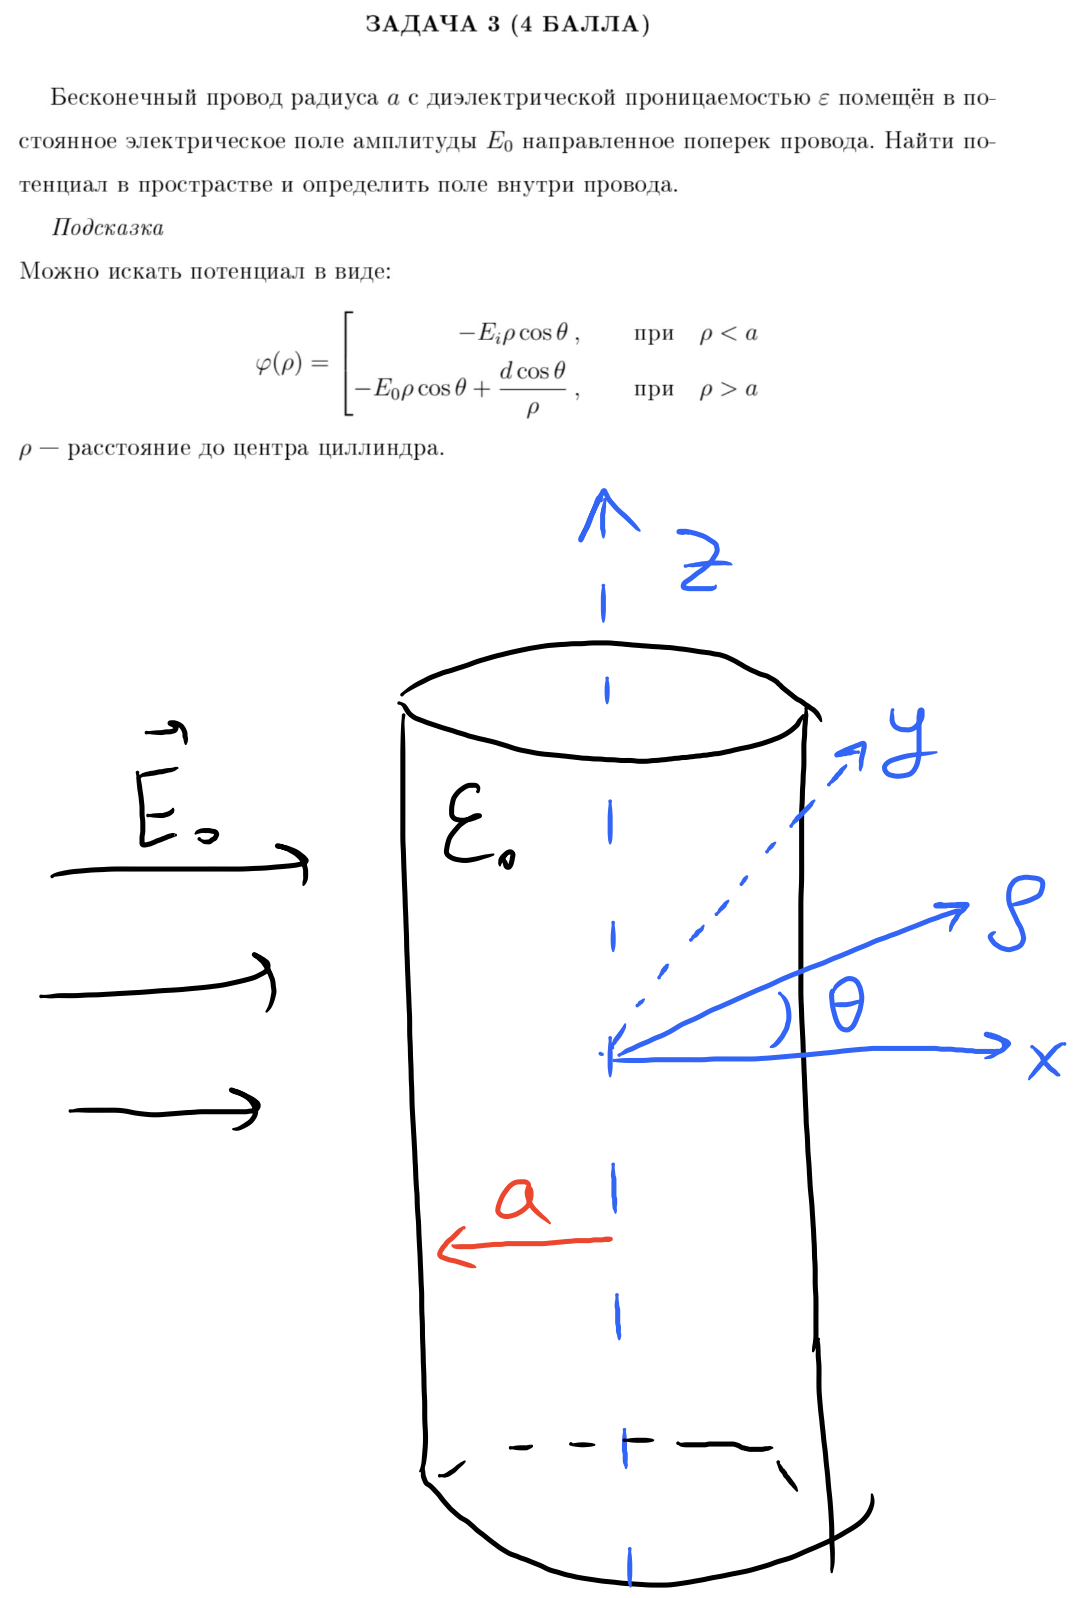
\includegraphics[width=1\textwidth]{photo.png}
%\begin{center}
%\underline{Рисунок 1}:
%\end{center}
\par Решение:
\par
\par Пункт (а). $\chi_{ijk}^{(2)}$ - всего 27 компонент
\par Все $C_2$ - симметрии:
%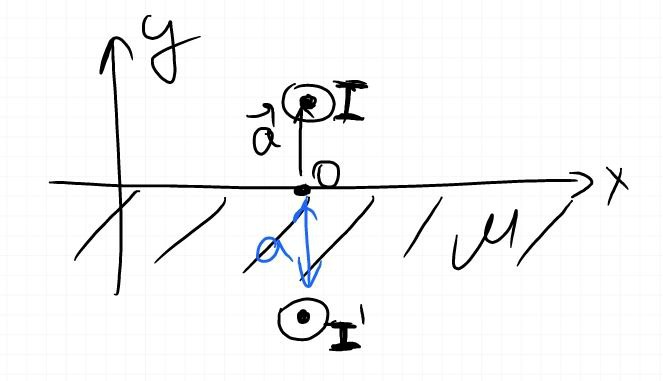
\includegraphics[width=1\textwidth]{photo_1.jpg}
%\par
%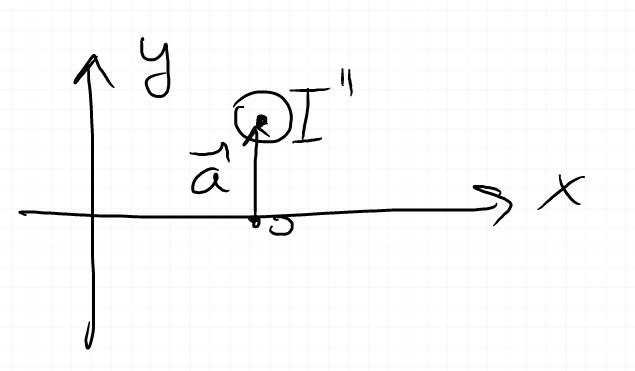
\includegraphics[width=1\textwidth]{photo_2.jpg}
\par Поворот на $\pi$ вокруг $x$:
\[
    x \rightarrow x, \,\,\, y \rightarrow -y, \,\,\, z \rightarrow -z
\]
\[
    p_x \rightarrow p_x, \,\,\, p_y \rightarrow -p_y, \,\,\, p_z \rightarrow -p_z
\]
\[
    E_x \rightarrow E_x, \,\,\, E_y \rightarrow -E_y, \,\,\, E_z \rightarrow -E_z
\]
\par Получаем:
\[
    \left.
    \begin{array}{r}
        p_x = \chi_{xxy}^{(2)} E_x E_y \\
        p_x = \chi_{xxy}^{(2)} E_x (-E_y)
    \end{array}
    \right\} \Rightarrow \chi_{xxy}^{(2)} = 0
\]
\par Ан-но:
\[
    \chi_{xxy}^{(2)} = \chi_{xyx}^{(2)} = \chi_{xxz}^{(2)} = \chi_{xzx}^{(2)} = 0
\]
\par Ан-но $\pi$ вокруг $y$:
\[
    \chi_{yxy}^{(2)} = \chi_{yyx}^{(2)} = \chi_{yxz}^{(2)} = \chi_{yzx}^{(2)} = 0
\]
\par Ан-но $\pi$ вокруг $z$:
\[
    \chi_{zxy}^{(2)} = \chi_{zyx}^{(2)} = \chi_{zxz}^{(2)} = \chi_{zzx}^{(2)} = 0
\]
\par Все $C_3$ симметрии вокруг диагоналей:
\[
    x \rightarrow y, \,\,\, y \rightarrow z, \,\,\, z \rightarrow x
\]
\[
    \chi_{xyz}^{(2)} = \chi_{yzx}^{(2)} = \chi_{zxy}^{(2)}
\]
\[
    \chi_{xzy}^{(2)} = \chi_{zyx}^{(2)} = \chi_{yxz}^{(2)}
\]
\[
    \chi_{xxx}^{(2)} = \chi_{yyy}^{(2)} = \chi_{zzz}^{(2)}
\]
\[
    \chi_{xyy}^{(2)} = \chi_{yzz}^{(2)} = \chi_{zxx}^{(2)}
\]
\[
    \chi_{xzz}^{(2)} = \chi_{yxx}^{(2)} = \chi_{zyy}^{(2)}
\]
\par Вокруг другой диагонали
\[
    x \rightarrow -z, \,\,\, y \rightarrow x, \,\,\, z \rightarrow -y
\]
\par Получаем:
\[
    \chi_{iii}^{(2)} = \chi_{ijj}^{(2)} = 0
\]
\par Отражение $\sigma$ отн диагонали грани
\[
    x \rightarrow x, \,\,\, y \rightarrow z, \,\,\, z \rightarrow y
\]
\par Тогда все $\chi_{ijk}^{(2)}$ с разными индексами равны. По сути это можно переписать через перестановку индексов:
\[
    \chi_{xyz}^{(2)} = \chi_{\sigma\{x; y; z\}}^{(2)}
\]
\par Ответ:
\[
    \chi_{xyz}^{(2)} = \chi_{\sigma\{x; y; z\}}^{(2)}
\]
\[
    \chi_{iii}^{(2)} = \chi_{\sigma\{i; i; j\}}^{(2)} = 0
\]
\par Один линейно-независимый элемент
\par Пункт (б) я не решал
\end{large}
\end{document}
